\section{电话}\label{sec:10-8}

电话是人们生活中常用的通讯工具(图 \ref{fig:10-37})。
最简单的电话装置是由话筒、电池组和听筒组成的。
话筒、电池组和听筒串联在电路里(图 \ref{fig:10-38})。

\begin{figure}[htbp]
    \centering
    \begin{minipage}{6cm}
    \centering
    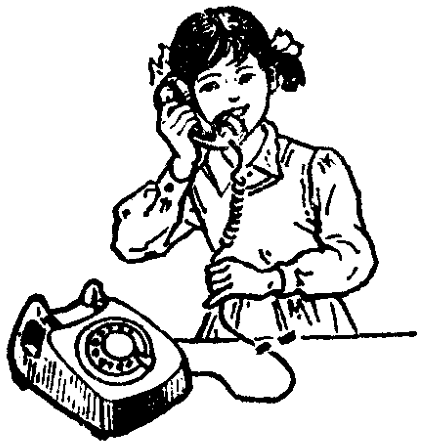
\includegraphics[width=5cm]{../pic/czwl2-ch10-37}
    \caption{}\label{fig:10-37}
    \end{minipage}
    \qquad
    \begin{minipage}{8cm}
    \centering
    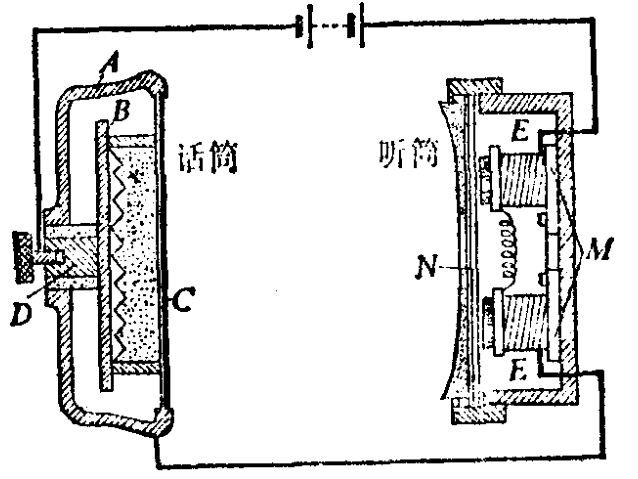
\includegraphics[width=7cm]{../pic/czwl2-ch10-38}
    \caption{}\label{fig:10-38}
    \end{minipage}
\end{figure}


话筒是一个圆形的金属盒 $A$,盒上面有一个碳精薄片——振动膜 $C$。
盒里面装一个碳精盘 $B$,在碳精盘和振动膜中间装满了碳粒。
碳精盘跟一个露出盒外的金属柱 $D$ 连着,金属柱 $D$ 跟金属盒 $A$ 是绝缘的。
话筒里的碳粒接触得并不紧密,有较大的电阻,如果被压紧,电阻将减小。

你可能会注意到,声音是由物体的振动而产生的。
当胡琴、提琴等乐器上的弦发声的时候,它们的弦都在振动。鼓被敲响的时候,鼓膜也在振动。
当我们对着话筒的振动膜说话的时候,声带的振动就会引起空气的振动,空气的振动使话筒的振动膜做相应的振动。
振动膜的振动就使里面的碳粒发生忽松忽紧的变化,它的电阻就发生忽大忽小的变化,这时电路中就通过忽弱忽强的电流。

在听筒里面有一个永磁铁 $M$, 在磁铁的两极上面套着螺线管 $E$,螺线管的两头连到电路里。
在磁极的前面有一个薄铁片 $N$,这就是听筒的振动膜。
当电路中的忽强忽弱的电流通过听筒里的螺线管的时候,磁铁对听筒振动膜的吸力就发生忽大忽小的变化。
振动膜在这种忽大忽小的力的作用下就振动起来。
听筒振动膜的振动情形跟话筒振动膜的振动情形是一样的。
所以我们就听到跟话筒前面的讲话相同的声音。

上面讲的电话装置只是用来说明电话的基本原理。
实际应用的电话机,每一台都是既有话筒又有听筒,另外还有电铃等附属设备。
随着科学技术的飞速发展,新型电话机不断出现,使人们使用起来越来越方便。

